\documentclass[12pt, a4paper]{article}
\usepackage[T1]{fontenc}
\usepackage[utf8]{inputenc}
\usepackage[spanish]{babel}
\usepackage[margin = 1cm]{geometry}
\usepackage{listings}
\usepackage{xcolor}
\usepackage{parskip}
\usepackage{url}
\usepackage{anysize}
\usepackage[hidelinks]{hyperref}
\usepackage{amsmath}	
\usepackage{graphicx}
\usepackage{multirow}

\definecolor{codegreen}{rgb}{0,0.6,0}
\definecolor{codegray}{rgb}{0.5,0.5,0.5}
\definecolor{codepurple}{rgb}{0.58,0,0.82}
\definecolor{backcolour}{rgb}{0.95,0.95,0.92}

\lstdefinestyle{mystyle}{
	backgroundcolor=\color{backcolour},   
	commentstyle=\color{codegreen},
	keywordstyle=\color{magenta},
	numberstyle=\tiny\color{black},
	stringstyle=\color{codepurple},
	basicstyle=\ttfamily\footnotesize,
	breakatwhitespace=false,         
	breaklines=true,                 
	captionpos=b,                    
	keepspaces=true,                 
	numbers=left,                    
	numbersep=7pt,                  
	showspaces=false,                
	showstringspaces=false,
	showtabs=false,                  
	tabsize=2
}

\lstset{style=mystyle}

\lstdefinelanguage{pseudocode}{
    morekeywords={Inicio, Fin, Escribir, Leer, Variables},
    sensitive=false,
    morecomment=[l]{//},
    morestring=[b]"
}

\title{\textbf{
	\begin{flushright}
		Capítulo II
	\end{flushright}
	ALGORITMOS Y PROGRMAS ELEMENTALES
	}}
\date{\today}
\author{Las Chicas Superpoderosas}

\begin{document}
\maketitle
\renewcommand{\contentsname}{}
\tableofcontents

\newpage

\section{Los problemas algorítmicos}

Todo problema es un problema algorítmico, pues todo problema requiere de una secuencia ordenada de pasos a seguir para resolverlo, esta secuencia además de orden exige lógica en su proceder; pero los problemas a los que se harán referencia en este libro son aquellos que se han de resolver empleando algoritmos computacionales.
Los algoritmos se representarán empleando Pseudocódigo y se llevarán al computador mediante el lenguaje de programación PYTHON, para ello se empleará el editor PyScripter (\textcolor{blue}{\url{http://pyscripter.software.informer.com}}), su instalación sobre Windows es sumamente sencilla, en el site anterior se encuentran las ayudas necesarias sobre el uso e instalación del IDE, el PyScripteres un entorno de desarrollo integrado para PYTHON, que corre sobre Windows; es libre y de código abierto, está construido en Object Pascal. Para resolver un problema computacional se debe en primer lugar analizar la situación a la que esta enfrentandose el desarrollador, en segundo lugar, y luego de un analisis objetivo se diseñará la solución del problema, seleccionando la secuencia lógica más corta y de menos uso de recursos (de computador) a seguir para resolver el problema estudiado, este algoritmo se representará en Pseudocódigo (puede ser representado de otras maneras, ver capítulo I), por último se implementará la solución en PYTHON.

\subsection{Análisis del problema}
Es Primordial comprender y eneteder de que se trata el problema para poder determinar una solución adecuada, claro esta decir que el analisis de la situción a la que enfrenta el desarrollador deberá determinar si el planteamiento del problema cuenta con la información suficiente como para poder llegar a una solución.
La pregunta clave es: ¿Qué datos se necesita conocer para determinar una solución al problema? Por ejemplo: si se desea calcular S, donde S se define como:
\[
    S = \dfrac{x^3}{\sqrt{x}}
\]
Entonces se debe conocer $x$ para efectuar los calculos, además se puede observar en el denominador $x$ debe ser un entero positivo, en cuento a la respuesta S este debe ser un valor real. Joyanes (2003) menciona que en el análisis del problema se deben determinar tres cosas:

\begin{enumerate}
    \item[a.] Las \textbf{entradas} (los datos [que se trabajarán como variables de entrada] necesarios para alimentar un proceso y originar una salida de información satisfactoria para el usuario o para el desarrollador)
    \item[b.] Las \textbf{salidas de información}, las cuales son consecuencia del proceso que soluciona el problema, la información de salida también se trata como variables de salida.
    \item[c.] \textbf{Variables} a usar en el proceso de solución al problema:
\end{enumerate}

\begin{center}
    variables de entrada + variables de salida \\[2cm]
\end{center}

\subsection{Pseudocódigo}
Es un lenguaje que permite describir con claridad y exactitud los pasos a seguir para resolver el problema, es decir permite describir el algoritmo (proceso que da solución al problema), este no es un lenguaje de programación, sin embargo su estructura es muy similiar a la de un lenguaje estructurado de computadoras, si bien es cierto las primeras versiones estaban en ingles, actualmente el Pseudocodigo se ha llevado a diferentes idiomas humanos, con la finalidad de hacer más entendible el diseño de un algoritmo computacional. Ejemplo:

\textbf{PROBLEMA:} Se desea mostrar en pantalla la suma de
dos números ingresados por teclado.

\textbf{ANÁLISIS:} Se desea sumar dos valores y el resultado mostrarlo en pantalla se necesitarán dos valores como entradas mientas que como salida será la suma de ambos.

\begin{center}
    Ejemplo en Pseudocódigo
\end{center}

\begin{lstlisting}[language = pseudocode, caption = {Algoritmo en Pseudocódigo}]
//Algoritmo: Suma de dos numeros

Inicio del Programa

Variables: numero_1, numero_2, resultado <- 0 

Escribir "Ingrese un numero: "
Leer numero_1
Escribir "Ingrese otro numero: "
Leer numero_2

resultado <- numero_1 + numero_2

Escribir "El resultado de la suma es: ", resultado

Fin del Programa

\end{lstlisting}

\textbf{Nota:} El simbolo $\leftarrow$ se le denomina operador de asignación. La traducción del agoritmo representado en Pseudocodigo.

Ahora en un lenguaje de programación de alto nivel como \textbf{Python} el algoritmo es directa:

\begin{center}
    Ejemplo en Python
\end{center}

\lstinputlisting[language = Python, caption = {Código en Python}]{Codigo en Python/suma_de_numeros.py}

\textbf{Nota:} El simbolo \# sirve para colocar comentarios en un programa en PYTHON (un comentario será una porción de escritura dentro del código que el intérprete de PYTHON ignorará al momento de ejecutarse el programa).

El input() permite el ingreso de datos al programa, pero en tipo string (cadena de caracteres) por ello se coloca int(input()) para que lo que se capture con input() se convierta a valor entero. Línea 4 y 5 del ejemplo de Python.

El valor entero se asigna a la variable. En PYTHON no es necesario declarar el tipo de datos de la variable a emplear. Si se desea capturar un valor real, se emplea float() analogamente a como se empleó int() en el ejemplo.

El texto \textquotedbl{\textbackslash {n}\textquotedbl} da un salto de línea en el programa.

\section{Estructura de un programa en PYTHON}
Un programa en PYTHON no tiene una estructura tan formalizada como el C/C++ o en Java, quizás una de las características de un programa en este lenguaje es el empleo de las tabulaciones(indentación), ejemplo: el siguiente programa tiene por objetivo mostrar como PYTHON hace uso estricto de las tabulaciones.

\textbf{Problema:} Se pide el ingreso de un caracter, y determina si es número, letra mayúscula, letra minúscula, o un simple caracter.

\begin{center}
    Ejemplo en Python
\end{center}

\lstinputlisting[language = Python, caption = {Código en Python}]{Codigo en Python/caracter.py}

\textbf{Nota:} Un carácter leído desde el teclado como un carácter, para ser comparado como número ASCII (\textcolor{blue}{\url{https://theasciicode.com.ar/}}), se usa ord(), esta función devuelve el valor número de un carácter, si se desea obtener el carácter de un valor númerico, se utiliza la función chr(), por ejemplo print(chr(78)) nos mostraría en la salida del  programa "N".
Observe que el uso de la tabulación es esctricto en Python, de no considerarse, la tabulación, el intérprete de Python mostraría error en la ejecución. 

\newpage
\begin{center}
	Ejemplo de un programa con error de tabulación en Python.
\end{center}

\lstinputlisting[language = python, caption = {Código de error de Python}]{Codigo en Python/error_caracter.py}

El error que marcaria el intérprte Python por no considerar las tabulaciones es:

\begin{verbatim}
	line 7
    print("El caracter es un numero")
    ^
Error de sangría: se esperaba un bloque con sangría después de la 
declaración 'if' en la línea 6
\end{verbatim}

Por tanto, se puede decir con seguridad que este lenguaje es muy ordenado y exige al desarrollador al escribir un código fuente.

\subsection{Programa de computadora}
Un programa de computadora es la implementación, en un determinado lenguaje de programación, de un algoritmo diseñado para obtener un resultado.

Niklaus Wirth, quien desarrolló el lenguaje de programación Pascal tiene un libro titulado:

\begin{center}
	``Algoritmos + Estructuras de Datos = Programas``
\end{center} 

En este título se puede resumir con simplicidad el asunto de todo el estudio de la programación de computadoras. 
Los programas de computadora pueden ser lineales, cuando no existen condiciones que separen el flujo secuencial del programa en más de un escenario posible, y pueden ser no lineales cuando sucede lo contrario del concepto anterior. 
Un programa es considerado por algunos desarrolladores como un proceso por el cual se transforman las entradas (datos de entrada) en salidas (información de salida)

\newpage

\begin{figure}
	\centering
	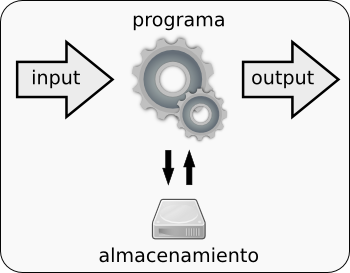
\includegraphics[width = 6cm]{Figuras/input y output.png}
	\caption{input y output}
	\label{i_o}
\end{figure}

\textbf{Nota:} Las salidas de un programa, para ser consideradas válidas, deben tener significado para el quién usa o necesita del mencionado programa, de lo contrario, y muy a pesar de que el algoritmo este bien definido, no se podrá decir que se trate de un programa válido.

\subsection{Programas básicos}
Antes de comenzar a trabajar resolviendo algoritmos se
debe hacer un hincapié en los principios de la programación en PYTHON, ya que es el lenguaje en que se implementarán los mencionados algoritmos que se ha de diseñar. PYTHON fue diseñado para ser entendido de manera sencilla y fácil. Una de las características más resaltantes de este lenguaje es el empleo de palabras en lugar de símbolos, haciendo más sencilla la programación y la traducción del algoritmo al lenguaje, también el NO EMPLEO de las para separar bloques de código, ejemplo:

\begin{table}[h!]
	\centering
	\begin{tabular}{|lll|}
	\hline 
	\multicolumn{3}{|p{342.5297pt}|}{\centering Cálculo de la suma de los números pares e impares de manera separada, de los números enteros positivos comprendidos entre 1 y 50.}\\ 
	\hline 
	\multicolumn{1}{|p{114.4275pt}}{\multirow [t]{3}{=}{\centering C/C++}} & \multicolumn{1}{|p{114.4275pt}}{\multirow [t]{3}{=}{\centering PHP}} & \multicolumn{1}{|p{113.67469pt}|}{\multirow [t]{3}{=}{\centering PYTHON}}\\ 
	
	\multicolumn{1}{|l}{} & \multicolumn{1}{|l}{} & \multicolumn{1}{|l|}{}\\ 
	
	\multicolumn{1}{|l}{} & \multicolumn{1}{|l}{} & \multicolumn{1}{|l|}{}\\ 
	\hline 
	
	\end{tabular}
\end{table}

\subsection{Entrada y salida en un programa PYTHON}

\section{Programas de secuencia lineal}

\end{document}